\section*{Теорема Менгера. Форма Гёринга}


    \begin{theorem}[]
        Пусть $X,Y \subset V(G)$, причём $X \not \subset Y$ и $Y \not \subset X$. Известно, что $|X| \geq k, |Y| \geq k, \kappa(X,Y) \geq k$. Тогда существуют $k$ непересекающихся путей из $X$ в $Y$.
    \end{theorem}
    \begin{proof}[Доказательство] 
        \hfill \begin{itemize}
            \item Индукция по размеру графа.
            \item Для всех меньших графов считаем, что утверждение доказано. 
        \end{itemize}
         
    \textbf{Случай 1}: \textit{существует разделяющее множество $R$ ровно из $k$ элементов}
    \begin{itemize}
        \item Во-первых, путь из $X$ в $R$ не проходит через множество $Y$, потому что иначе $R$ -- не разделяющее множество.
        \begin{figure}[h]
            \centering
            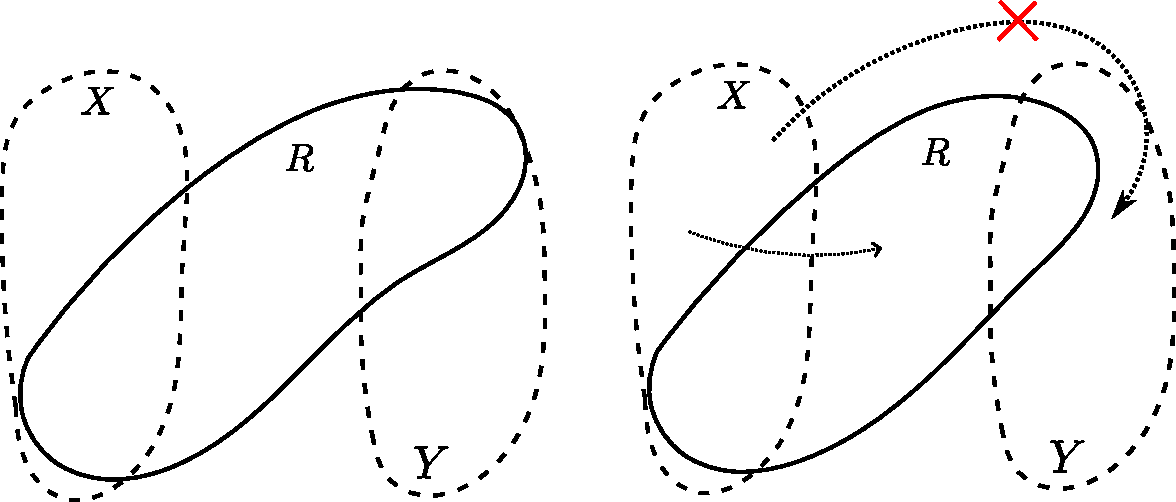
\includegraphics[width=0.7\textwidth]{images/menger1}
        \end{figure}
        \item Удалим из графа $Y \ \backslash \ R$. 
        \item Заметим, что в новом графе работает индукционное предположение для множеств $X$ и $R$: если $\kappa(X, R) < k$, то найдётся множество $S$, которое разделяет $X$ и $R$, а значит, разделяет и $X, Y$.
        \item Применяем И.П. для $X$ и $R$. Аналогично, для $R$ и $Y$.
        \item Так как вершин в $R$ ровно $k$, то полученные пути стыкуются и получаются $k$ непересекающихся путей. 
        \begin{figure}[H]
            \centering
            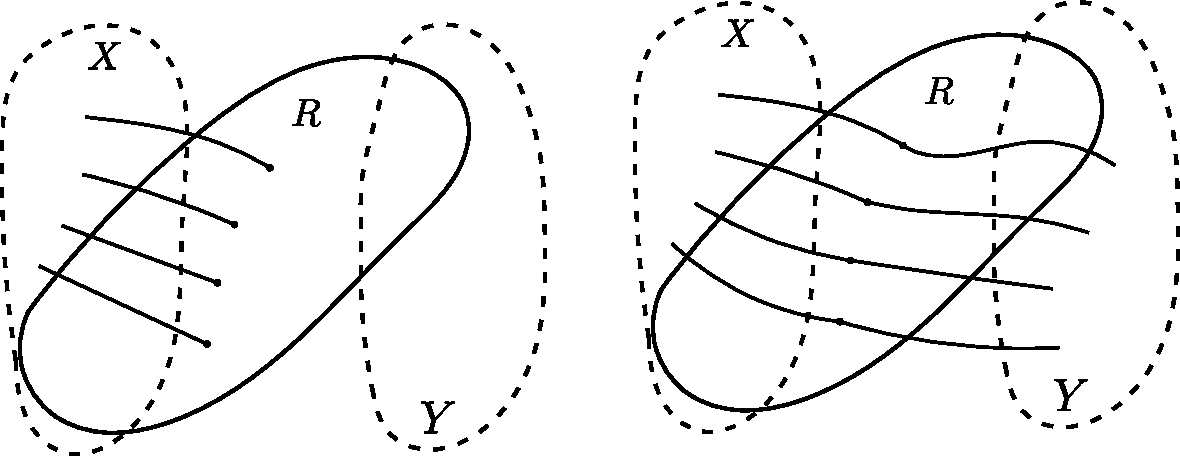
\includegraphics[width=0.7\textwidth]{images/menger2}
        \end{figure}
    \end{itemize}

    \textbf{Случай 2}: \textit{такого множества не существует}

    \begin{itemize}
        \item Тогда $\kappa(X,Y) > k \Rightarrow |R| > k$.
        \item Будем постепенно удалять рёбра в графе $G$.
        \item При удалении ребра $e = xy$ в $G$ возможны 3 случая:
            \begin{itemize}
                \item Мы убрали все рёбра (этот случай очевиден)
                \item Условие $\exists R: |R| = k$ начало выполняться (тогда мы тоже победили)
                \item Нашлось разделяющее множество $T$ размера меньше чем $k$ (в $G-e$)
            \end{itemize}
    \end{itemize}
    \begin{note}[о третьем случае]
        Дмитрий Валерьевич сам сказал, что Гёринг в своей статье написал что-то вроде <<ну, очевидно же, вы чего?>>, однако, как мы убедимся далее, этот случай является наиболее противным моментом во всей теореме.
    \end{note}

    Подробнее рассмотрим случай 3. В $G - xy$ найдётся $T: |T| < k$, тогда $T \cup \left\{ xy \right \}$ \textbf{разделяет} $X, Y$ в исходном $G$. Однако, как мы знаем, $T \cup \left\{ x \right \}$ и $T \cup \left\{ y \right \}$ \textbf{не разделяют} $X, Y$ в $G$ (так как $\kappa(X,Y) > k$).

    Повторим рассуждение ещё раз: итак, $T \cup \left\{ xy \right \} $ разделяет $X,Y$. Значит, по-хорошему путь должен в обязательном порядке проходить по ребру $xy$. Однако, $T \cup \left\{ x \right \} $ также удалит и ребро $xy$, причём не разделит множества $X,Y$.
    \begin{figure}[h]
        \centering
        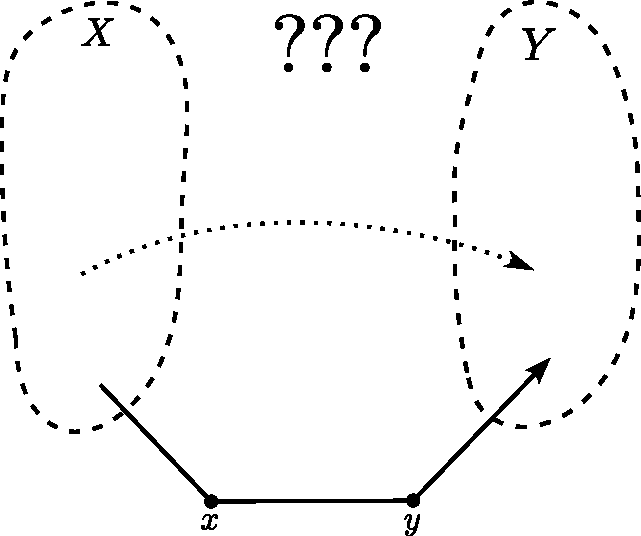
\includegraphics[width=0.4\textwidth]{images/menger-badcase}
    \end{figure}

    А это возможно лишь в одном случае: $T \cup \left\{ x \right \} $ полностью удаляет множество (НУО) $X$ в графе $G$, поэтому нужные нам пути существуют: нечего стало разделять.

    $X \ \backslash \ T$ непусто из-за того, что $|T| < k, |X| \geq k$. В то же время, $X \subset T \cup \left\{ x \right \}, |X| \geq k, |T \cup \left\{ x \right \}| \leq k$. Значит, $X = T \cup \left\{ x \right \}$.

    \pagebreak
    Проведём аналогичные рассуждения для вершины $y$ и множества $Y$ и получим, что $Y = T \cup \left\{ y \right \} $. В итоге получим следующую картинку:

    \begin{figure}[H]
        \centering
        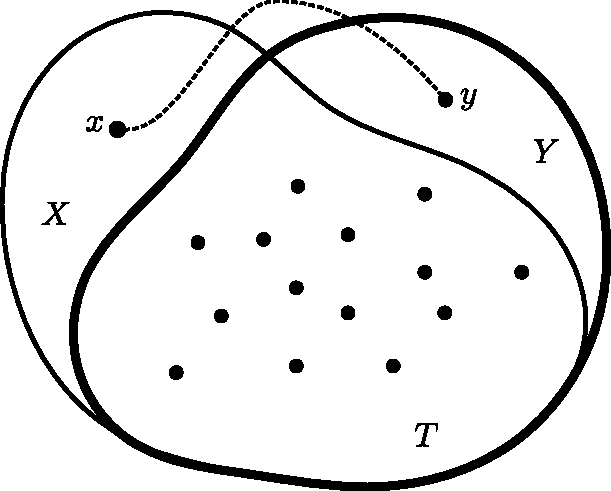
\includegraphics[width=0.5\textwidth]{images/menger_final}
    \end{figure}

    Теперь легко увидеть $k$ нужных нам путей в графе $G$: это вершины множества $T$ (вырожденные пути, все вершины $T$ общие для $X, Y$) и ребро $xy$.

    Итого, мы рассмотрели все 3 случая и полностью доказали теорему.
\end{proof}
